%%%%%%%%%%%%%%%%%%%%%%%% HIGS Beam time Request Document %%%%%%%%%%%%
% Author M.W. Ahmed
%%%%%%%%%%%%%%%%%%%%%  DO NOT EDIT THE FOLLOWING LINES %%%%%%%%%%%%%
\documentclass[titlepage,twoside,letterpaper,12pt]{article}
 \usepackage{apacite} 
 \usepackage{fancyhdr}
\usepackage{color}
\usepackage{csquotes}
\setlength{\evensidemargin}{0.5cm}
\setlength{\oddsidemargin}{0.5cm}
\setlength{\textwidth}{17cm}
\setlength{\textheight}{20cm}
\setlength{\topmargin}{0.3cm}

\usepackage{graphicx}
\pagestyle{fancy}
\usepackage{wrapfig}
\fancyhf{}
\rhead{AutoVis}
\lhead{Project Proposal - Final Dissertation}
\rfoot{Page \thepage}

\begin{document}
\begin{titlepage}
%%%%%%%%%%%%%%%%%% COVER SHEET %%%%%%%%%%%%%% Please Fill %%%%%%%
{\noindent{\large{ \underline{\bf{Proposal Information}}}}}\\ \vskip 0.25in
\noindent{{Proposal Title: \bf{AutoVis - Automated Visualisation using Machine Learning}}}\\
\newline
{\large{ \underline{Student Information:}}}\\
Name : Muhammad Abdullah Akmal\\
Email: b7031482@my.shu.ac.uk - agfa.94@gmail.com\\
Telephone: +44 7568922477\\
Module: MSc Big Data Analytics\\
\newline
{\large{ \underline{Supervisor Information:}}}\\
Name : Dr. Christopher R Roast \\
Email: c.r.roast@shu.ac.uk\\
Telephone: +44 1142256845\\
\vskip 3.00in
\begin{figure}[!h]

\includegraphics[scale=2.00]{Figures/AUTOVIS_logo.png}

\includegraphics[scale=0.25]{Figures/shefield4.png}
\end{figure}

\newpage
\tableofcontents
\listoffigures

%{\large{Beam Information}} \\
%Total Hours of Beam on target:\\
%Please provide a list of desired deam setting pararmeters:\\
%\begin{table}[h]
%\vspace{0.1in}
%\begin{center}
%\begin{tabular}{|c|c|c|c|c|} \hline 
%E$_{\gamma} (MeV)$  & Collimator Size (mm) & Flux on target  & Polarization & Hours \\ \hline  
%\end{tabular}
%\end{center}
%\end{table}

%\begin{titlepage}
%\centering
%\vskip 0.1in
%%%%%%%%%%%%%%%%%%%%%% PROPOSAL STARTS HERE %%%%%%%%%
%
%{\Large{\bf{This is an Example Title. Please Enter the Title of Your Experiment Here}}}
%
%%%%%%%%%%%%%%%%%%%%%%%%%%%%%%%%%%%%%%%%%%%%%%%%%%%%%%%%%%%%%%%%%%%%%
%\vskip 0.5in
%%%%%%%%%%%%%%%% Enter the Spokesperson and Collaborator Info %%%%%%%
%{\large{First Author (Spokesperson), Next Author, Next Author}} \\
%{\em{Institution Name and Address}}  
%\vskip 0.2in
%{\large{Next Author, Next Author (Spokesperson-Contact), Next Author}} \\
%{\em{Institution Name and Address}} 
%\vskip 0.2in
%{\large{Next Author, Next Author, Next Author}} \\
%{\em{Institution Name and Address}} 
%\vskip 0.2in
%{\large{Next Author, Next Author, Last Author}} \\
%{\em{Institution Name and Address}} 
%%%%%%%%%%%%%%%%%%%%%%  DO NOT EDIT THE FOLLOWING LINE %%%%%%%%%%%%%%
%\vskip 0.2in
%\large{\today}
\end{titlepage}

%%%%%%%%%%%%%%%%%%%%%%%%% Summary %%%%%%%%%%%%%%%%%%%%%%%
\section{Problem Statement}
\begin{displayquote}
"Automatic generation of graphics/visuals from the raw dataset by identifying the structure of dataset using machine learning techniques."
\end{displayquote}

To explain further, this problem is divided two folds:
\begin{enumerate}
\item Collection of datasets that machine learning could be used upon identifying the structure. 
\item Then use of machine learning to train a model that can learn the rules of visualisation (mapping from decision matrix to visualisation language).
\end{enumerate}

\begin{figure}[!h]
\centering
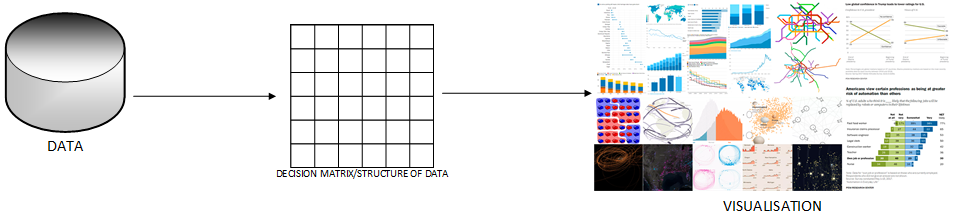
\includegraphics[scale=0.65]{Figures/1.png} 
\caption{Project Diagram}
\label{fig:1}
\end{figure}

%%%%%%%%%%%%%%%%%%%%%%%%% Project Description %%%%%%%%%%%%%%%%%%%%%%%
\section{Objectives}

Following are the main objectives intended to achieve during this project:
\begin{enumerate}

\item Collection of datasets which machine learning algorithms can used to train an algorithm.

\item Creation of Decision matrix depending upon the structure of datasets using Neural network. This matrix will contain the information about the what kind of visualisation might be useful for the specific kind of data.

\item Creation of Model that automatically select the subset of fields for visualisation (generally datasets have several fields which cannot be concurrently visualised). This Model would help to identify the differences between different data types. Data can be of any type namely string, numeric, temporal, ordinal, categorical etc. Moreover, applying transformations depending upon the data type e.g. aggregate transform function can be applied to numeric data but cannot to string data. Finally, the model must translate the decision matrix to a visualisation language like vega-lite \cite{Satyanarayan} etc. 
\end{enumerate}

\section{Introduction}

Visualisation is divided into two sub fields, scientific visualisation and information visualisation. Scientific visualisation deals with the scientific data which involves spatial component e.g. 3D medical imagery etc. while information visualisation deals with the data that doesn’t involve the spatial factor e.g. weather forecast, document data etc. \cite{Tory}. 

Information visualisation is defined by Card, Mackingly and Shneiderman (Card, Mackinglay, and Shneiderman, 1999) as the tool of visualisation for amplification of human cognitive abilities. Information visualisation is referred as “Visual Data Mining” \cite{Frenay}, since humans are particularly good at identifying outliers and trends via visualisation \cite{AnneTreisman}.

Machine learning and information visualisation both somehow deal with the better understanding for user via visualisation and analysis of dataset. Machine learning is basically used for finding pattern in large datasets \cite{Frenay}. Combining both fields can help in Computationally enhanced visualisation \cite{Rayar}, visually enhanced mining techniques and Integrated Visualisation and mining possibilities.

We mainly will deal in this project with the information visualisation and its automation using the machine learning.

\section{Motivation}
Majority of the advanced automated visualisation are based on heuristics. Heuristics are set of basic rules which are use to make decisions and judgments about specific  It would be great if they can learn the patterns by itself and follow them to improve upon the previous ones. Best visualisation to the user can increase the sense of understanding regarding that specific data. Most of the time in data mining and analysis process is spend in data visualisation and understanding. If this step is done automatically, it will save alot of process time and resources consumption.  Intent of this project is in relation with effective visualisation, automation in visualisation and deep learning neural network. 
The idea behind this research is to come up with a method which reduces the user role in the data visualisation. Machine learning will play its role by reducing the user only to select data descriptions and may be to some extent identify the algorithms and automatically everything is done by computer. Later, it may be users may be given a set of visualisation from which specific selection can be made.

\section{Literature Review}
Generally, before diving into the data for specific usage, analysists use data visualisation techniques to understand the data. For that they use different range of tools starting from the completely abstract tools, easy to learn and fast to make visualisations e.g. Microsoft excel, Google Sheets are easy to use but have limited functionalities. While, some of them require expertise and give more appropriate results e.g. HTML canvas and OPENGL gives the better results but require programming expertise to achieve it \cite{Dibia} as shown in figure \ref{fig:flow}.

\begin{figure}[!h]
\centering
\includegraphics[scale=0.65]{Figures/flow.png} 
\caption{Flow of visualisation from speed to expressiveness}
\label{fig:flow}
\end{figure}

Declarative Languages basically forms a logical and methodological framework for program and system. It uses propositional techniques based on rational concepts for specifying the properties and objects. \cite{Broy}. They are like a tradeoff between others. You get enough speed and expressiveness \cite{Wickham}. But they might be difficult to understand the syntax and cope with the level of abstraction adopted. Plus, they might have some re-usability issues e.g. for non-R (the programming language) users it might be difficult to understand ggplot2 etc. 

One of the key issues in the visualisation is the scalability. Humans cannot perceive the knowledge when more than a few combined features are put together. Moreover, there perception is limited in between 2 and 3 dimensions. In real time, its really difficult to compute large datasets interactively. This is where machine learning comes in. Ml provides with the ability to automatically summarize or compress the big data solutions via clustering and projection methods \cite{bridginginformation}. Connecting ML with IV(Information Visualisation), we can somehow resolve the human perception problem and interactivity issues.

Artificial Neural Networks(ANN) are computing system which are inspired from the  biological neurological system of animals. These system have an ability to learn from its past experiences, gain on it progressively and help in automatic decision making process using the improved knowledge \cite{appliedNN}. It consists of neurons. These are divided into different layers and they can send signals to each others in the form of 0's and 1's. 

If there are multiple layers between input and output layer then such ANN is called Deep Neural Networks (DNN). They are usually deepforward networks, i.e. they move from input to output, with different weights attached to neurons. If they can move in any direction then such networks are called Recurrent Neural Networds (RNN), they consist of memory Long-short term memory (LSTM), which allows it to store information while propagation \cite{RNN}.

DNN's surpasses the machine translation system performance, as compared to phrase based approach. DNN's used large datasets which help in appropriate model fitting. Different approaches already have been employed in industry to translate the domain specific languages and programming languages, try to make system learn to write imporoved code \cite{decode}. Data2Vis \cite{Dibia}, used the RNN seq2seq to directly translate the source and target. \cite{reverse} used the CNN (Convolutional Neural Networks) for the classification of type of graphical markers (e.g. bars, lines, areas, points etc.). This classification was further used to encode data in the chart. This encoding is used to recover visual encoding specification. They used OCR alongside it also.

%DeepDive, Yago and EntityCube are some of the examples of corpus building which extracts the data and by the help of Deep NLP tools from the web and then create knowledge base systems \cite{deepdive}. 


Just to gain more insight the next subsection will go through the related work done.

\subsection{Related Work}
BOZ is an automated visualisation tool used for designing of the task-oriented graphics and presentation of these graphics. BOZ allows the users to draw the logical conclusion from the set of graphics and help in streamlining this information depending upon the search of the users \cite{Casner}. It only uses analytical approach that combines set of heuristics to reach to the required searched information. These set of heurisics can help us to understand what rules are used to identify the data. Which ultimately can help in building the decision matrix.

Interactive visualisation is really important when we deal with data exploration. To acheive that Vizdeck model can prove to be helpful.VizDeck \cite{Key} is a self-organising dashboard for visual analytics. By looking at the statistical properties of the data, it recommends the appropriate visual analytics. A prototype card games adopts these recommendations and organises the interactive visual dashboard in no time without any programming.  
To bring on the automation, the working of APT can be really helpful in the current scenario. APT (A Presentation Tool) is a porotype model create for automated designing of the graphical presentation by clearly defining graphical language that explains the syntactic and semantic properties of the graphical presentation. \cite{Mackinlay}. AI was used in implementation of this prototype and most of the design is generated using the compositional algebra which includes the compositional operators and primitive graphical languages. It deals with the 2D static presentations automations like bar chart, scatter plot, connected graphs etc.

SAGE \cite{Roth}, an automated presentation designing system, which takes as an input the data characteristics and primitive knowledge about the visualisation intentions. By incorporating SageBrush (graphics are construct using the primitives about the design or partial design) and SageBook (browser for retrieving previously created images). SAGE inherit functionalities from other systems like APT, BOZ and ANDD (Automated Network Diagram designer, which takes the network model and set of design directives as an input and produces network diagram \cite{Marks}).

Data2Vis (a web-based prototype), uses LSTM-based neural translation model which formulate the seq2seq translation, train it and then generate visualisation \cite{Dibia}. Data2Vis gives the understanding how deep learning models can be used to identify the structure via visualisation languages.

\section{Dataset}
\cite{reverse} generated the dataset using the Vega Visualisation grammer by automatically generating the charts, collecting the charts from the Quartz (a news website) and RDataset. We will try to follow the same methodoly. RDataset \cite{R-DataSet} is available automatically, vega files \url{https://github.com/victordibia/data2vis/tree/master/bin/tools}. It consists of the 1147 datasets distributed in the statistical software and software packages. By using the compass recommendation engine \cite{compass} on 11 different dataset vega specification charts will be created and by using the python we will extract different charts from the Quartz website. This is an approximate estimation of chart corpus that would be available to us after the processing table \ref{tab:1}

\begin{table}[h]
\vspace{0.1in}
\begin{center}
\begin{tabular}{|c|c|c|} \hline 
& \textbf{Vega Charts} & \textbf{Quartz} \\ \hline  
\textbf{Area Charts} & 477 &0 \\
\textbf{Bar Charts} &1358 &191 \\
\textbf{Line Charts} &360 &283 \\
\textbf{Scatter Plots} &2123 &1 \\ \hline
\textbf{Total} & \textbf{4,318} & \textbf{475} \\ \hline
\end{tabular}
\end{center}
\caption{Approximately Estimated Chart Corpus}\label{tab:1}

\end{table}

\section{Research Methodology}
Top-Down(Deductive) approach will be utilised in this project implementation as shown in the figure \ref{fig:life}.

\begin{figure}[!h]
\centering
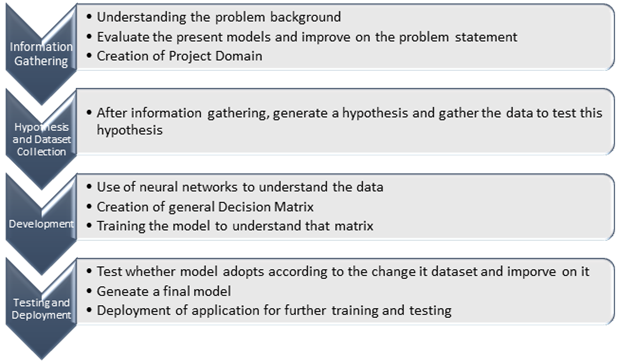
\includegraphics[scale=0.65]{Figures/lifecycle.png} 
\caption{Cycle of adopted Research Methodology}
\label{fig:life}
\end{figure}

Following are the steps:
\begin{enumerate}
\item Understand the problem background
\item Generate Dataset
\item Start generic Testing to understand the data and applying different machine learning techniques
\item Test and Evaluate the present solution
\item Mature hypothesis
\item Generate Decision Matrix
\item Model Creation and Testing
\item Deployment
\item Validation with Unknown Dataset via deployed application

\end{enumerate}

Intention is to start in maturing the problem statement, alongside generating the dataset and go through more research understanding the implementation of the current system discussed in the section ‎5.1. After that Mature the hypothesis, generate the decision matrix which contains information about the visualisation of data. This decision matrix will further be used to fit a model. Using cross validation, it would be tested and this step is repeatable to achieve better results. After that we will move towards the deployment and testing of the final system.

We basically rely on the Deep Learning algorithms of machine learning to create decision matrix and then built on that to understand and visualise the data. Literature shows the seq2seq, LSTM neural translation accompanying with RNN (Recurrent Neural Network) and Vega-lite may be an approach to this problem. Generating this model, training it and deploying to validation and further improvements will be last and final step. 


\section{Timeline}
Following Gant Chart shows the initial workplan to complete the project and division into different tasks as shown in the figures \ref{fig:timeline_1} and \ref{fig:timeline_2}.

\begin{figure}[!h]
\centering
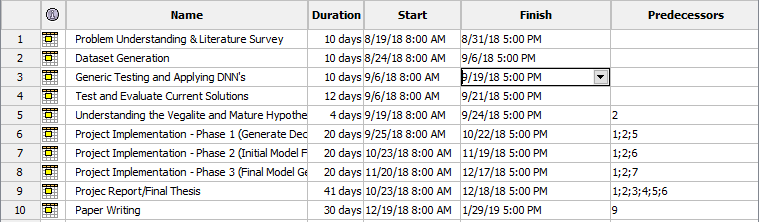
\includegraphics[scale=0.65]{Figures/timeline_1.png} 
\caption{Task divisions and Temporary Deadlines}
\label{fig:timeline_1}
\end{figure}
\begin{figure}[!h]
\centering
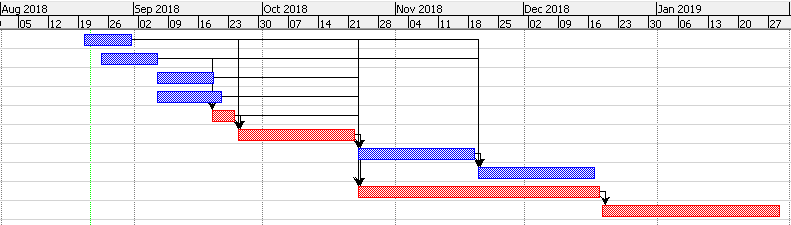
\includegraphics[scale=0.65]{Figures/timeline_2.png} 
\caption{Gantt Chart}
\label{fig:timeline_2}
\end{figure}


\section{Potential Outcome}
We intend to come up with deep neural network approach like RNN multi sequential with long-short term memory, building on the previous knowledge. This would be able to successfully convert the set of data into a knowledgeable matrix which can be further used to take visualisation decisions. Moreover, for testing/validation we intend to create a prototype web or software-based application that would be able to perform three operations:
\begin{itemize}
\item	Importing the data (potentially in JSON)
\item	Generate Visualisation
\item	Update Visualisation (applying different transformation functions)
\end{itemize}
\section{Advantages}
This research project can help in following lines:
\begin{itemize}

\item	It will enable user to create insightful visualisation with less or no programming.
\item	It will help in handy, fast and escalate the visualisation capabilities of users.
\item	Analysists can use it for initial understanding of the data and then adopting the algorithms according to the results, speeding up the process for them.
\item	It will help in understanding the structure of data which is unusual or unknown.
\item	It can help in exploring the data which is complex, saving the effort of going through applying different visualisation techniques and then reaching to the one that makes sense.
\end{itemize}

\section{Challenges}
Following are the likely challenges in this project:
\begin{itemize}
\item	Tackling the unstructured data, training, modelling and visualisation must be one of the challenges.
\item	Collection of data and making the machine learning algorithms to understand this data is a big challenge.
\item	Automatically selection of attributes would be one of the challenges
\item	Incorporation of different data visualisation techniques at one place may be 
something achievable but might prove to be tedious work.
\end{itemize}

\section{Ethics and Conduct}
Meaningful visualisation results in increase of knowledge and understanding in the relevant problem. This can help in future prediction which can help in more improve decision in that field. Since, visualisation is the cognitive process which is under research, so it is difficult to come up with ethical guide to visualisation but some of the ethics that should be considered by the designers while creating graphics:
\begin{itemize}
\item	Visualisations are intended to bring attention to relevant matter.
\item	Visualisations are based on thorough analysis of information.
\item	Visualisation are built in a way that are easy to comprehend.
\item	Selection of meaningful, clear, efficient and in-depth informative graphic that makes sense to the viewer rather than selecting one which a designer likes or easy to implement \cite{Cairo}.
\item	Things like hierarchy of visual properties and appropriate labelling must be kept in mind while designing \cite{Skau}.
\item	Depict the data and analysis in accurate way.
\item	Clearly exposing to different visualisation techniques and remain open to criticism.
\item	Visualisation shouldn’t be intentionally used for hiding or confusing the truth. It shall not misguide the uninformed. 
\item	Designer shall remain fully responsible for virtual and actual meaning portrayed by the graphics.

\end{itemize}
\bibliographystyle{apacite} % We choose the "plain" reference style
\bibliography{ref} % Entries are in the "refs.bib" file



%\begin{thebibliography}{99}
%\bibitem{latexcompanion}
%Reference One {\textit et al.}, Phys. Rev. {\bf C0}, 999 (2000).
%\end{thebibliography}
\end{document}
